\documentclass[tikz,border=4pt]{standalone}
\usepackage{tikz}
\usepackage{amsmath}
\usetikzlibrary{positioning,arrows.meta,shapes.geometric,fit}

\begin{document}
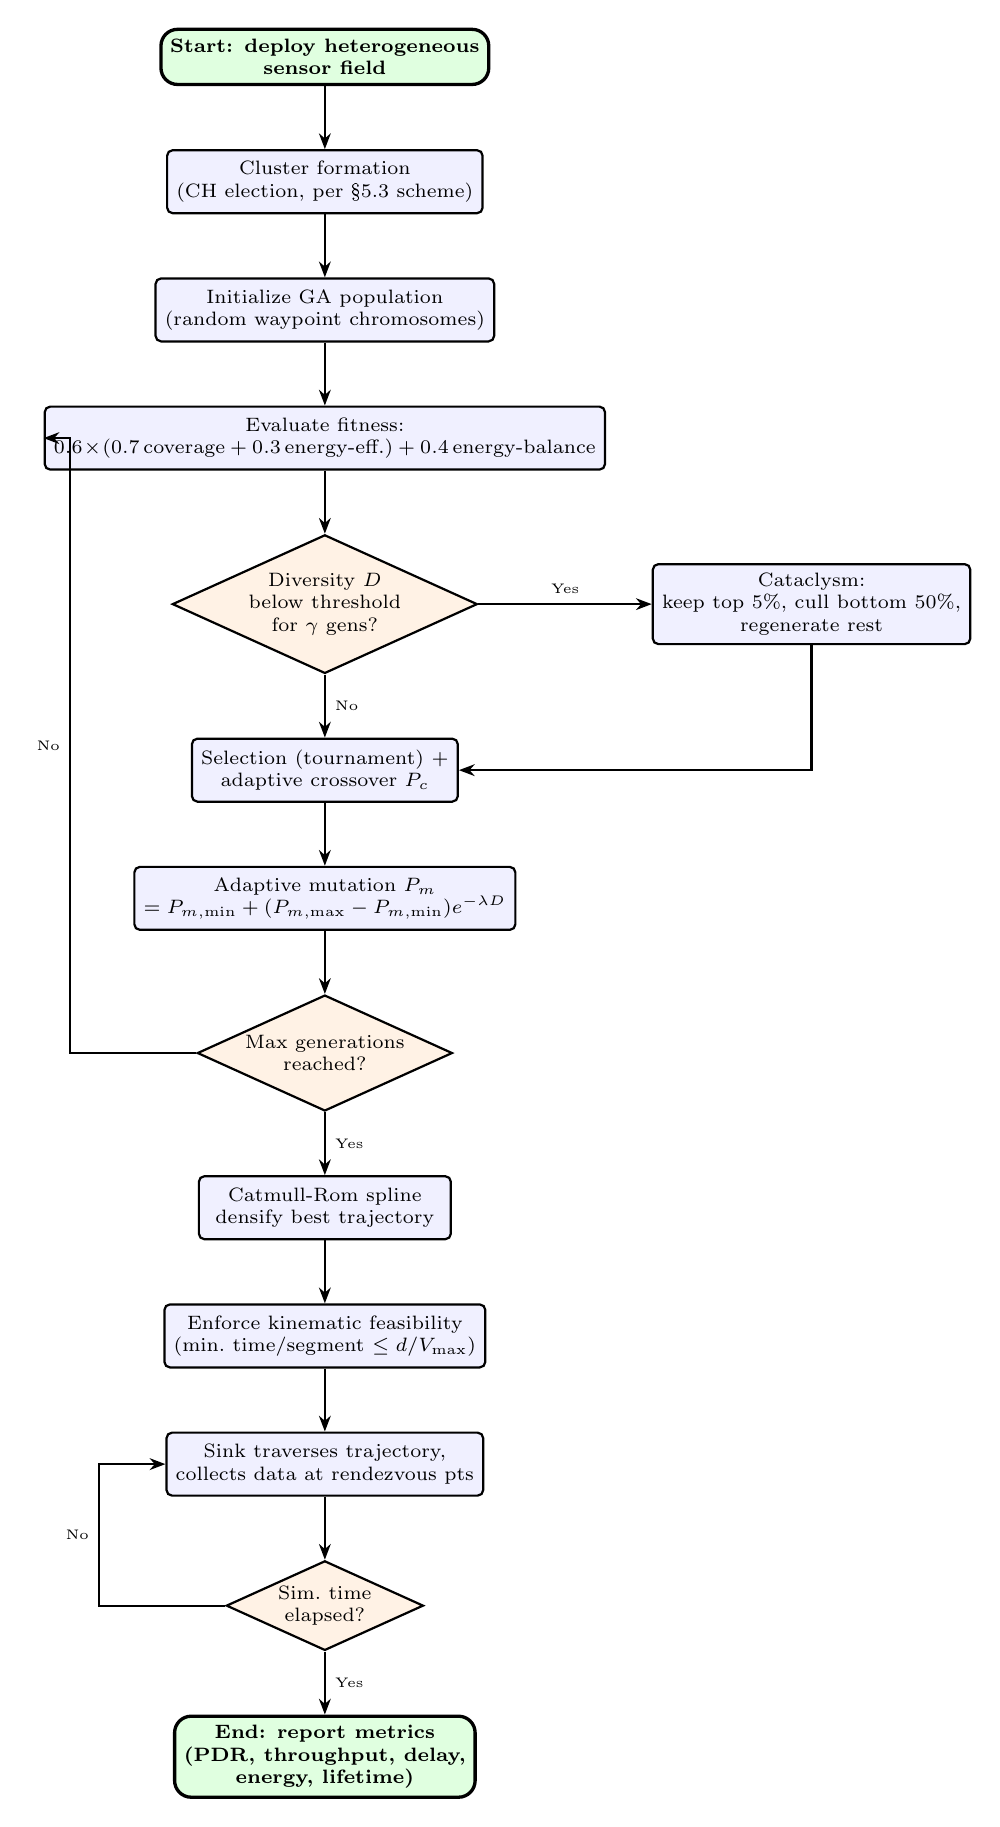
\begin{tikzpicture}[
    node distance=8mm and 14mm,
    box/.style={rectangle, draw, thick, rounded corners=2pt, align=center, minimum width=32mm, minimum height=8mm, font=\scriptsize, fill=blue!6},
    decision/.style={diamond, draw, thick, aspect=2.2, align=center, font=\scriptsize, fill=orange!10, inner sep=1pt},
    startstop/.style={rectangle, rounded corners=6pt, draw, very thick, align=center, minimum width=28mm, minimum height=7mm, font=\scriptsize\bfseries, fill=green!12},
    arr/.style={-{Stealth[length=2mm]}, thick}
]

\node[startstop] (start) {Start: deploy heterogeneous\\sensor field};
\node[box, below=of start] (cluster) {Cluster formation\\(CH election, per §5.3 scheme)};
\node[box, below=of cluster] (init) {Initialize GA population\\(random waypoint chromosomes)};
\node[box, below=of init] (fitness) {Evaluate fitness:\\$0.6\!\times\!(0.7\,\text{coverage}+0.3\,\text{energy-eff.}) + 0.4\,\text{energy-balance}$};
\node[decision, below=of fitness] (diversity) {Diversity $D$ \\below threshold\\for $\gamma$ gens?};
\node[box, right=of diversity, xshift=8mm] (cataclysm) {Cataclysm:\\keep top 5\%, cull bottom 50\%,\\regenerate rest};
\node[box, below=of diversity] (select) {Selection (tournament) +\\adaptive crossover $P_c$};
\node[box, below=of select] (mutate) {Adaptive mutation $P_m$\\$= P_{m,\min}+(P_{m,\max}-P_{m,\min})e^{-\lambda D}$};
\node[decision, below=of mutate] (termcheck) {Max generations\\reached?};
\node[box, below=of termcheck] (spline) {Catmull-Rom spline\\densify best trajectory};
\node[box, below=of spline] (kinematic) {Enforce kinematic feasibility\\(min.\ time/segment $\le d/V_{\max}$)};
\node[box, below=of kinematic] (traverse) {Sink traverses trajectory,\\collects data at rendezvous pts};
\node[decision, below=of traverse] (roundcheck) {Sim.\ time\\elapsed?};
\node[startstop, below=of roundcheck] (endnode) {End: report metrics\\(PDR, throughput, delay,\\energy, lifetime)};

\draw[arr] (start) -- (cluster);
\draw[arr] (cluster) -- (init);
\draw[arr] (init) -- (fitness);
\draw[arr] (fitness) -- (diversity);
\draw[arr] (diversity) -- node[right, font=\tiny]{No} (select);
\draw[arr] (diversity) -- node[above, font=\tiny]{Yes} (cataclysm);
\draw[arr] (cataclysm) |- (select.east);
\draw[arr] (select) -- (mutate);
\draw[arr] (mutate) -- (termcheck);
\draw[arr] (termcheck.west) -- ++(-16mm,0) |- node[near start, left, font=\tiny]{No} (fitness.west);
\draw[arr] (termcheck) -- node[right, font=\tiny]{Yes} (spline);
\draw[arr] (spline) -- (kinematic);
\draw[arr] (kinematic) -- (traverse);
\draw[arr] (traverse) -- (roundcheck);
\draw[arr] (roundcheck.west) -- ++(-16mm,0) |- node[near start, left, font=\tiny]{No} (traverse.west);
\draw[arr] (roundcheck) -- node[right, font=\tiny]{Yes} (endnode);

\end{tikzpicture}
\end{document}
